\documentclass[a4paper]{scrreprt}

% Uncomment to optimize for double-sided printing.
% \KOMAoptions{twoside}

% Set binding correction manually, if known.
% \KOMAoptions{BCOR=2cm}

% Localization options
\usepackage[english]{babel}
\usepackage[T1]{fontenc}
\usepackage[utf8]{inputenc}

% Sub figures
\usepackage{subcaption}

% Quotations
\usepackage{dirtytalk}

% Floats
\usepackage{float}

% Enhanced verbatim sections. We're mainly interested in
% \verbatiminput though.
\usepackage{verbatim}

% Automatically remove leading whitespace in lstlisting
\usepackage{lstautogobble}

% CSV to tables
\usepackage{csvsimple}

% PDF-compatible landscape mode.
% Makes PDF viewers show the page rotated by 90°.
\usepackage{pdflscape}

% Advanced tables
\usepackage{array}
\usepackage{tabularx}
\usepackage{longtable}

% Fancy tablerules
\usepackage{booktabs}

% Graphics
\usepackage{graphicx}

% Current time
\usepackage[useregional=numeric]{datetime2}

% Float barriers.
% Automatically add a FloatBarrier to each \section
\usepackage[section]{placeins}

% Custom header and footer
\usepackage{fancyhdr}

\usepackage{geometry}
\usepackage{layout}

% Math tools
\usepackage{mathtools}
% Math symbols
\usepackage{amsmath,amsfonts,amssymb}
\usepackage{amsthm}
% General symbols
\usepackage{stmaryrd}

% Utilities for quotations
\usepackage{csquotes}

% Bibliography
\usepackage[
  style=alphabetic,
  backend=biber, % Default backend, just listed for completness
  sorting=ynt % Sort by year, name, title
]{biblatex}
\addbibresource{references.bib}

\DeclarePairedDelimiter\abs{\lvert}{\rvert}
\DeclarePairedDelimiter\floor{\lfloor}{\rfloor}

% Bullet point
\newcommand{\tabitem}{~~\llap{\textbullet}~~}

\pagestyle{plain}
% \fancyhf{}
% \lhead{}
% \lfoot{}
% \rfoot{}
% 
% Source code & highlighting
\usepackage{listings}

% SI units
\usepackage[binary-units=true]{siunitx}
\DeclareSIUnit\cycles{cycles}

\newcommand{\lecture}{62079 - Statistical Learning Methods with R}
\newcommand{\series}{2}
% Convenience commands
\newcommand{\mailsubject}{\lecture - Series \series}
\newcommand{\maillink}[1]{\href{mailto:#1?subject=\mailsubject}
                               {#1}}

% Should use this command wherever the print date is mentioned.
\newcommand{\printdate}{\today}

\subject{\lecture}
\title{Series \series}

\author{Michael Senn \maillink{michael.senn@students.unibe.ch} --- 16-126-880}

\date{\printdate}

% Needs to be the last command in the preamble, for one reason or
% another. 
\usepackage{hyperref}

\begin{document}
\maketitle


\setcounter{chapter}{\numexpr \series - 1 \relax}

\chapter{Series \series}

\section{Plotting education vs wage}

The figure below shows the relationship between education and wage. The
outliers were eliminated beforehand.

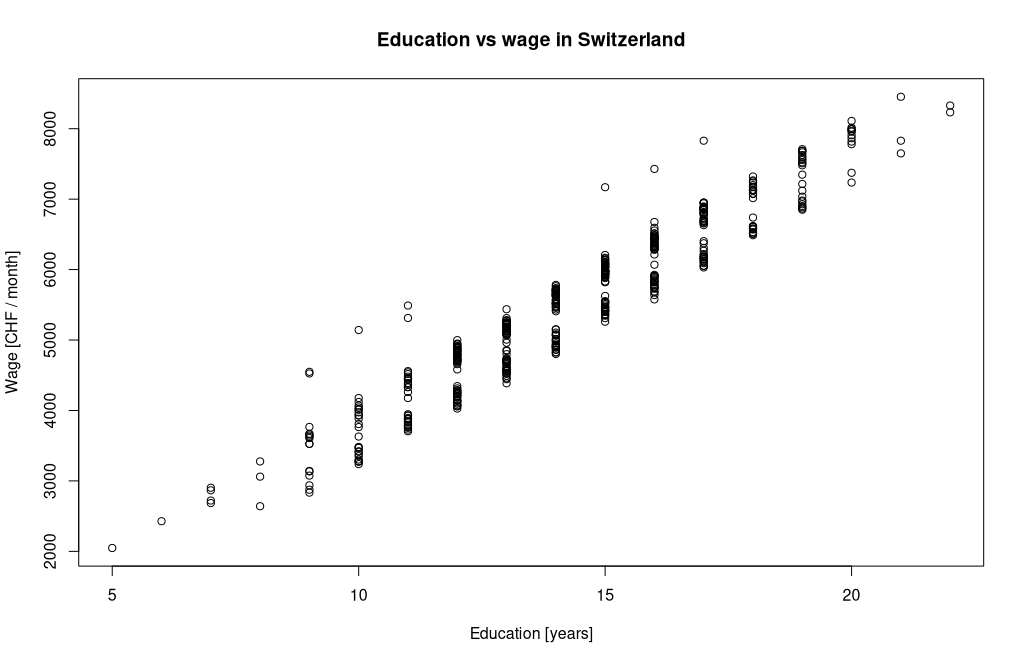
\includegraphics[width=\textwidth]{resources/01_education_wage.png}

\section{Plotting education vs wage per gender}

The figure below shows the relationship between education and wage, grouped by
gender. The outliers were eliminated beforehand.

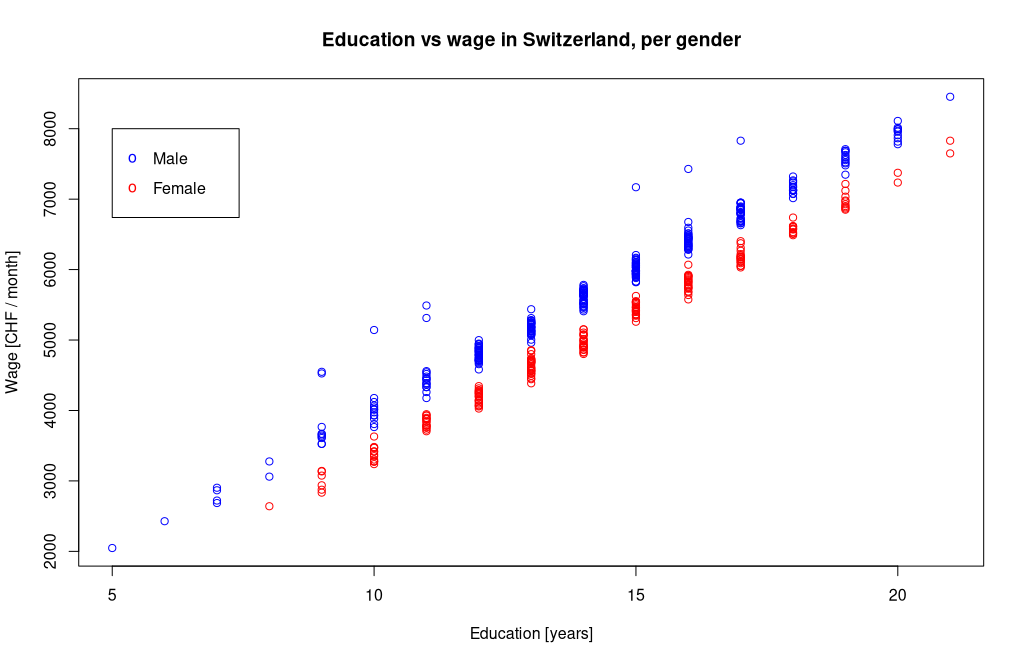
\includegraphics[width=\textwidth]{resources/02_education_wage_gender.png}

\section{Treating unknown tumours}

Table \ref{tbl:treating_unknown_tumours} shows the success ratio of drug- and
surgery-based treatments, given no further information.

\begin{table}
		\centering
		\begin{tabular}{llll}
				\toprule
				Treatment & Cured & Failed & Success ratio \\
				\midrule
				Drugs   & 761     & 239    &    \SI{76.1}{\percent} \\
				Surgery & 658     & 342    &    \SI{65.8}{\percent} \\
				\bottomrule
		\end{tabular}
		\caption{Success ratios of drug- and surgery-based treatments of tumours of unknown size}
		\label{tbl:treating_unknown_tumours}
\end{table}

Given a tumour of unknown size, the recommended treatment would arguably be a
drug-based one. The reason for that is that, out of 1000 drug treatements,
761 were successful, for a success ratio of \SI{76}{\percent}. Surgeries on the
other hand were only successful in \SI{66}{\percent} of applications.

\section{Treating small tumours}

Table \ref{tbl:treating_tumours_known_size} shows the same ratios, but grouped
by the size of the treated tumours. Using the success ratio as a metric once
more, it is now more advisable to try surgery, with a success ratio of
\SI{89.5}{\percent}, rather than drugs, with a success ratio of
\SI{82.0}{\percent}.

\begin{table}
		\centering
		\begin{tabular}{lllll}
				\toprule
				Treatment & Tumour size & Cured & Failed & Success ratio \\
				\midrule
				Drugs     & Small       & 671   & 147    &    \SI{82.0}{\percent} \\
				Drugs     & Large       & 90    & 92     &    \SI{49.5}{\percent} \\
				Surgery   & Small       & 94    & 11     &    \SI{89.5}{\percent} \\
				Surgery   & Large       & 564   & 331    &    \SI{63.0}{\percent} \\
				\bottomrule
		\end{tabular}
		\caption{Success ratios of drug- and surgery-based treatments of tumours of known size}
		\label{tbl:treating_tumours_known_size}
\end{table}

\section{Treating large tumours}

Again referring to table \ref{tbl:treating_tumours_known_size}, the preferred
treatement based on the success ratio would be surgery with \SI{63.0}{\percent}
over drugs with \SI{49.5}{\percent}.

\section{Explaining the discrepancy}

This is interesting insofar as, with no additional information, the drug-based
therapy seems preferrable. However for both small as well as large tumours,
surgery seems to perform better.

Intuitively this seems paradoxical, as knowledge of the size of the tumour ---
no matter what the actual size is --- not only improves the probability of
success, but in fact completely changes which treatment should be utilized.

An understanding can be gained by looking at the distribution of samples. Most
samples of drug-based treatments are with small tumours, whereas most samples
of surgery-based treatments are with large tumours. As such the overall success
ratio of drug-based treatment is dominated by small tumours, whereas the one of
surgery is dominated by large tumours.

It now so happens that, for both drugs and surgery, the success ratio of small
tumours is larger than that of large tumours. As such the overall success ratio
of drugs exceeds the one of surgery, even though surgery actually has a better
chance of success for either size.

\end{document}
